% TinyAudit: 4-page short paper for the NeurIPS Responsible AI workshop (Oct 2026).
% Build: pdflatex tinyaudit_workshop.tex (twice, for references and figure refs).
%
% Style file: this paper uses the standard NeurIPS style. Download the workshop's
% style file (usually neurips_2026.sty, or the workshop's own variant) into this
% directory. If the workshop ships its own .sty, change the \usepackage line below.
% The [final] option shows author names; switch to no option for anonymous review
% if the workshop requires it. If the style file is absent, the paper falls back
% to a plain single-column layout so the draft still builds.
%
% Figures: expects figures/decoupling.pdf and figures/compression.pdf, generated by
%   python experiments/make_paper_figures.py
%
% References are embedded below via thebibliography, so no .bib file is needed.
% Only verified entries are cited.

\documentclass{article}

\newif\ifneuripsstyle
\IfFileExists{neurips_2026.sty}{%
  \neuripsstyletrue
  % The style file in this repo is the legacy pre-2000 NIPS macro set. It
  % declares no \DeclareOption/\ProcessOptions at all, so passing it any
  % option (including "final") makes the 2021+ LaTeX kernel hard-error with
  % "Unknown option ... for package neurips_2026" instead of just warning.
  % Load it bare and call \nipsfinalcopy directly instead; that is also a
  % no-op if a real modern neurips_2026.sty (which does handle [final]
  % itself) is dropped in later, since \nipsfinalcopy is idempotent.
  \usepackage{neurips_2026}%
  % \nipsfinalcopy switches the title block from the anonymous placeholder to
  % the real author names. It is defined by the style file loaded just above,
  % so it is always safe to call here in the file-present branch. Do NOT guard
  % it with \@ifundefined: an @-name written inside an \IfFileExists branch is
  % tokenized while @ is still a non-letter, which turns \@ifundefined into a
  % stray \@ and crashes with "You can't use \spacefactor in vertical mode".
  \nipsfinalcopy
}{%
  \neuripsstylefalse
  \usepackage[margin=1in]{geometry}%
  \usepackage{times}%
}

\usepackage[utf8]{inputenc}
\usepackage[T1]{fontenc}
\usepackage{hyperref}
\usepackage{url}
\usepackage{booktabs}
\usepackage{graphicx}
\usepackage{amsmath}
% microtype is deliberately omitted: with the legacy NeurIPS style's bitmap
% Helvetica (\font ... phvb), pdfTeX font expansion fails with "auto expansion
% is only possible with scalable fonts". It is typographic polish only. If you
% compile with a modern neurips_2026.sty and scalable fonts, you may re-add
% \usepackage{microtype} for slightly tighter justification.

% amsmath defines \And as a math operator; in the fallback layout we need it to
% behave like article's \and inside the author block. The NeurIPS style defines
% its own \And, so this only applies when the style file is absent.
\ifneuripsstyle\else
  \def\And{\and}
\fi

\title{TinyAudit: On-Device, Uncertainty-Aware Fairness Audits that Survive (and Expose) Compression}

\author{%
  Atharva Doke
  \And
  Kasyap Tumuluri
}

\begin{document}

\maketitle

\begin{abstract}
Machine learning is moving onto microcontroller-class hardware, where models are aggressively compressed (pruned, quantized) to fit. Responsible-AI audits, in contrast, are almost always run on full-precision models on a workstation, and they typically look at fairness, uncertainty, and explainability in isolation. We present TinyAudit, an auditing pipeline that measures all three together, through compression, and within the memory and compute envelope of the audited model itself. Using it we report two findings, each replicated and reported as a mean over 10 seeds. First, point-prediction fairness and calibration fairness are decoupled: the two lenses rank sensitive groups differently, so a model that looks fair on demographic parity need not be fair in its per-group calibration. The result holds on UCI Adult and replicates on COMPAS, whose favorable direction is inverted. Second, compression can hide unfairness: as a network is pruned it can look progressively fairer on demographic parity precisely as its calibration collapses, because it degrades toward a near-constant predictor. Finally, the audit is cheap enough to live on the device it inspects: its peak working set is about 0.6 MB plus 2.3 KB per audited sample, so streamed in small batches the whole pipeline runs under 1 MB and 0.1 s irrespective of test-set size.
\end{abstract}

\section{Introduction}

TinyML runs inference on microcontrollers with 32 to 512 KB of SRAM \cite{somvanshi2025}. To fit that budget, deployed models are pruned and quantized. The auditing tools that would check those models for fairness were built for a different world: cloud notebooks, full-precision weights, and demographic labels available at test time \cite{lee2021,deng2022,han2024}. Existing TinyML benchmarks measure latency, accuracy, and energy, but not fairness or explainability \cite{somvanshi2025}. The result is a gap. The models most likely to be compressed are the least likely to be audited, and when they are audited, the audit sees a model that is not the one deployed.

A second problem is that fairness audits usually stop at point predictions. A model can look fair on selection rates while its uncertainty is biased against a group \cite{kuzucu2024}, and abstaining on high-uncertainty inputs does not by itself repair group imbalance \cite{rosenblatt2024}. Uncertainty quantification now fits on KB-sized devices \cite{ghanathe2025}, but no existing system evaluates those estimates through a fairness lens, and no fairness toolkit fits on the device.

TinyAudit closes both gaps at once. It is a seven-stage pipeline that measures fairness, uncertainty, and explainability on the compressed model, inside a memory envelope sized for the device being audited. Our thesis: compression-era audits must be uncertainty-aware, because point fairness and calibration fairness are decoupled, compression can move one without the other, and all of this can be measured inside the device's own compute budget.

Contributions:
\begin{enumerate}
  \item An on-device audit instrument: a seven-stage pipeline coupling fairness, uncertainty, and explainability, measured on the compressed model, emitting a one-page traffic-light card and a machine-readable manifest.
  \item A decoupling result on UCI Adult, replicated on COMPAS with the favorable direction inverted (Section~\ref{sec:finding1}).
  \item Evidence that compression can hide unfairness: parity and calibration move in opposite directions under pruning (Section~\ref{sec:finding2}).
  \item A feasibility measurement: the audit's own peak working set is about 0.6 MB plus 2.3 KB per sample and is constant in test-set size when streamed (Section~\ref{sec:feasibility}).
\end{enumerate}

\section{The TinyAudit instrument}

TinyAudit takes a fitted model and a labeled test set and produces a one-page audit card plus a JSON manifest that every stage writes to. The card is generated from the manifest and never hand-edited; every figure in it is backed by a committed CSV. The stages, in order:

\textbf{1. Profile.} Parameter count, an analytic FLOPs proxy, peak RAM (via \texttt{tracemalloc}), and wall-clock per sample.
\textbf{2. Point fairness.} Demographic-parity difference (DP), equalized-odds difference (EO), and disparate-impact ratio (DI), each with an explicitly pinned favorable direction and a hypothesis-tested range.
\textbf{3. Uncertainty.} MC dropout (MLP only), a lightweight perturbation ensemble, and a QUTE-style early-exit estimator \cite{ghanathe2025}; each returns predictive entropy, variance, and mutual information.
\textbf{4. Uncertainty-aware fairness.} Per-group predictive entropy, per-group expected calibration error (ECE), and a selective-fairness AUC that integrates parity as low-confidence predictions are progressively abstained.
\textbf{5. Explainability.} SHAP, LIME, and a dependency-free occlusion explainer, cross-checked for top-feature flips across sensitive groups. SHAP and LIME are costly and fragile at the edge \cite{salih2025}, and embedded XAI needs design choices general-purpose toolkits do not automate \cite{nguyen2024}, which is why the occlusion explainer ships alongside them.
\textbf{6. Compression.} int8 dynamic quantization or magnitude pruning, applied \emph{before} every metric above, so the audit sees the deployed model.
\textbf{7. Render.} The one-page, traffic-light-coded card.

One design constraint shapes everything: the memory envelope. The audit's working set is dominated by per-sample buffers, so it can be streamed in small batches at a peak-RAM cost independent of test-set size (Section~\ref{sec:feasibility}). The whole public API is one call:

\begin{verbatim}
from tinyaudit import audit
card = audit(model=clf, data=(X_test, y_test), sensitive="sex",
             methods=["fairness", "uncertainty", "xai"], compression="int8")
card.to_pdf("adult_lr_int8.pdf")
\end{verbatim}

\section{Experimental setup}

\textbf{Datasets.} UCI Adult \cite{kohavi1996} (36{,}631 train / 12{,}211 test, 101 features after preprocessing; sensitive attributes sex and race), COMPAS \cite{angwin2016} (4{,}629 / 1{,}543, 5 features; on COMPAS the positive outcome is being flagged high-risk, so higher is worse), and the ACSIncome subset of Folktables \cite{ding2021} (146{,}748 / 48{,}917, 8 features, 2018 California). Adult and COMPAS are the near-universal fairness benchmarks \cite{fabris2022}; ACSIncome is the modern replacement for Adult's 1994 distribution \cite{ding2021}.

\textbf{Models.} Standard scikit-learn estimators fit on standardized features: logistic regression, an MLP with two hidden layers of 32 units, and a decision tree. Scaling matters: without it the Adult MLP sits near the majority-class rate (about 0.54 accuracy) versus about 0.84 with it. The scaler is fit on train only and applied outside the model, so compression and perturbation reach the raw weights.

\textbf{Reproducibility.} A single seed flag seeds \texttt{random}, NumPy, torch, and \texttt{PYTHONHASHSEED}. Every headline number is a mean $\pm$ std over seeds 0 to 9. Determinism is guaranteed on Linux/x86; elsewhere we expect last-digit float drift, which the std columns absorb. All models land in published ranges: Adult logistic regression reaches accuracy $0.852 \pm 0.003$ (ROC-AUC $0.906 \pm 0.002$) and the Adult MLP $0.837 \pm 0.003$ ($0.884 \pm 0.003$); on COMPAS the logistic model reaches $0.680 \pm 0.006$ ($0.731 \pm 0.008$) and the MLP $0.683 \pm 0.009$; on ACSIncome the MLP reaches $0.808 \pm 0.003$ ($0.889 \pm 0.002$). The fairness findings therefore sit on top of models that work, not on degenerate predictors.

\section{Finding 1: the fairness lenses decouple}
\label{sec:finding1}

Point-prediction fairness asks how often each group receives the favorable outcome. Calibration fairness asks how honest the model's confidence is per group. On the uncompressed logistic model, the two lenses rank the sensitive groups differently (Figure~\ref{fig:decoupling}).

\begin{figure}[t]
  \centering
  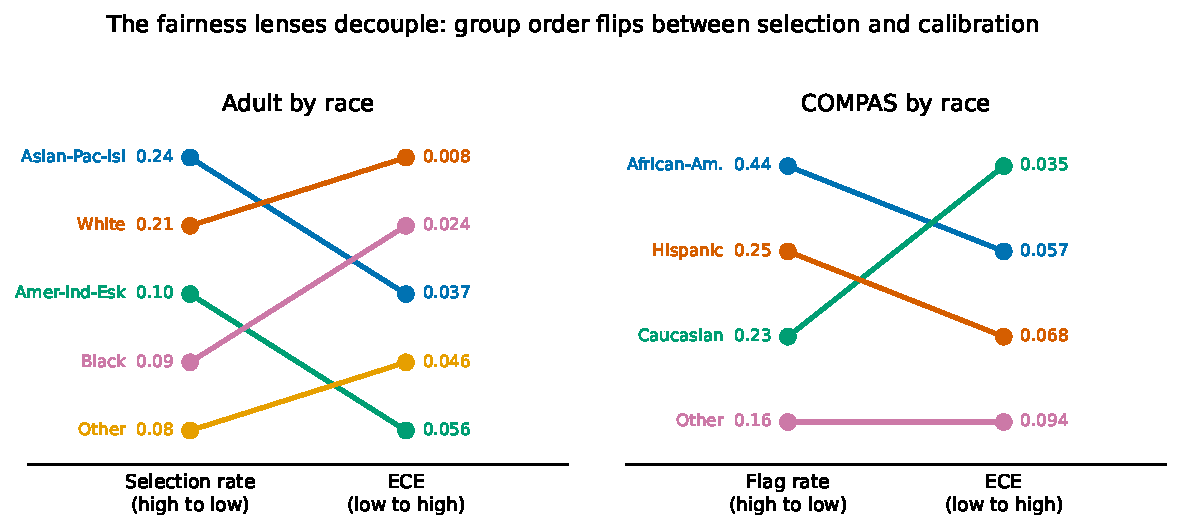
\includegraphics[width=\linewidth]{figures/decoupling.pdf}
  \caption{Finding 1. Rank slope charts for Adult (left) and COMPAS (right) by race, uncompressed logistic model, means over 10 seeds. Each line joins a group's rank by selection/flag rate to its rank by per-group ECE. Crossing lines mean the two lenses order the groups differently.}
  \label{fig:decoupling}
\end{figure}

\textbf{Adult by race} (five groups). By selection rate the ordering is Asian-Pacific-Islander ($0.240 \pm 0.014$), White ($0.207 \pm 0.005$), American-Indian-Eskimo ($0.098 \pm 0.026$), Black ($0.091 \pm 0.008$), Other ($0.081 \pm 0.024$). By calibration the ordering is different: White is only second-most-selected but by far the best calibrated (ECE $0.008 \pm 0.002$, three to seven times lower than every other group), while American-Indian-Eskimo is worst calibrated ($0.056 \pm 0.019$). The smaller groups carry higher, noisier calibration error that the selection view never surfaces.

\textbf{Adult by sex.} The gap is large in selection rate (Male $0.253 \pm 0.007$ vs Female $0.079 \pm 0.004$) but negligible in calibration (ECE $0.009 \pm 0.003$ vs $0.014 \pm 0.004$). The point view and the calibration view disagree again, this time in the opposite way: a big point disparity with no calibration disparity.

\textbf{COMPAS by race} (positive outcome = flagged high-risk; higher is worse; groups with $n<10$ dropped). African-American defendants are flagged at roughly twice the rate of the next group ($0.441 \pm 0.015$ vs Hispanic $0.249 \pm 0.046$), the well-known point disparity. Yet the worst-calibrated group, Other (ECE $0.094 \pm 0.029$), is the one flagged \emph{least} ($0.164 \pm 0.033$), and the best-calibrated group is Caucasian ($0.035 \pm 0.016$). The decoupling holds on a second dataset whose favorable direction is inverted, so it is not an Adult-specific label-convention artifact. The same pattern appears by sex: males are flagged more ($0.362 \pm 0.008$ vs $0.223 \pm 0.018$) but females are markedly worse calibrated (ECE $0.085 \pm 0.016$ vs $0.033 \pm 0.005$).

\textbf{Why it matters on-device.} Sensitive labels are rarely available at inference time on a deployed device, so on-device audit triggers lean on confidence scores as a proxy \cite{kenfack2024}. If the two lenses disagree about which group is worst served, a confidence threshold applied uniformly across groups can track the wrong disparity, consistent with the observation that uniform abstention can amplify imbalance \cite{rosenblatt2024} and that point metrics can mask biased uncertainty \cite{kuzucu2024}. Reporting both lenses is the cheap fix, and TinyAudit reports both by construction.

\section{Finding 2: compression can hide unfairness}
\label{sec:finding2}

\begin{figure}[t]
  \centering
  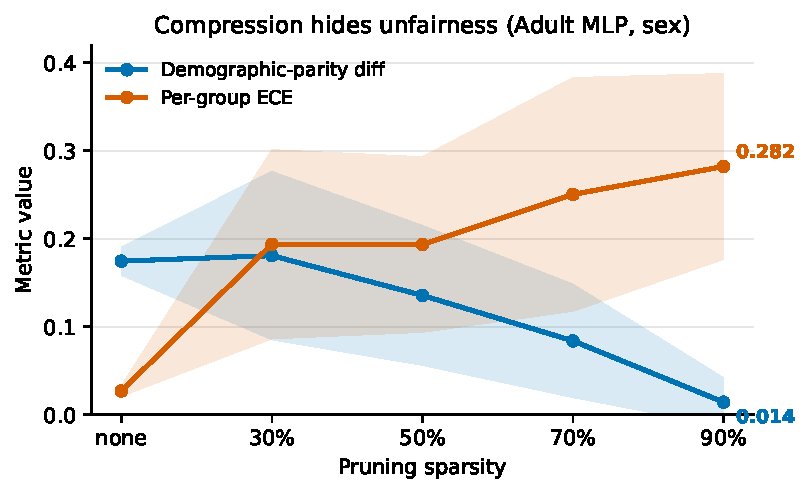
\includegraphics[width=0.8\linewidth]{figures/compression.pdf}
  \caption{Finding 2. Adult MLP by sex under magnitude pruning. Demographic-parity difference falls while per-group ECE climbs; bands are $\pm 1$ std over 10 seeds. The bands overlap at intermediate sparsities, so the robust claim is the endpoint contrast, not the middle ordering.}
  \label{fig:compression}
\end{figure}

We prune the Adult MLP to increasing sparsity and re-run the full audit at each level (Figure~\ref{fig:compression}). By sex, the demographic-parity difference falls from $0.175 \pm 0.016$ (unpruned) to $0.014 \pm 0.028$ at 90\% sparsity, a roughly 12-fold drop, while per-group ECE climbs from $0.027 \pm 0.006$ to $0.282 \pm 0.106$, a roughly 10-fold rise. By race the shape is the same: DP $0.150 \pm 0.024 \rightarrow 0.019 \pm 0.038$, ECE $0.051 \pm 0.007 \rightarrow 0.314 \pm 0.108$. The model looks fairer on parity precisely as its calibration collapses.

The mechanism is degradation toward a near-constant predictor. A near-constant predictor has a near-zero parity gap and is uniformly miscalibrated: parity ``improves'' for the worst possible reason. The corner case makes this vivid: the COMPAS logistic model at 90\% pruning (only about 5 features to begin with) predicts a single class for everyone and reports DP $= 0.000$, DI $= 1.000$, which is perfect parity by construction. We read those cells as an illustration of the mechanism, not a trend.

Two qualifications. First, intermediate pruning levels are seed-noisy (parity std of 0.06 to 0.10), so the robust claim is the direction between endpoints. Second, the effect is strongest where pruning actually damages the model. The logistic model barely degrades (DP $0.174 \pm 0.008 \rightarrow 0.126 \pm 0.014$, ECE $0.012 \pm 0.002 \rightarrow 0.026 \pm 0.004$ at 90\%), and correspondingly shows only a mild version of the effect. We also observe that int8 quantization can wreck calibration on its own; because int8 models' float weights are unreachable, their uncertainty columns are reported as missing rather than silently approximated, and temperature scaling on the audit set is a plausible mitigation.

The upshot for auditors: an audit that checks only demographic parity, run only after compression, would report the pruned model as the \emph{fairest} in the sweep. An uncertainty-aware audit flags the same model as the most broken.

\section{Feasibility: the audit fits on the device}
\label{sec:feasibility}

The novelty claim is not just that these metrics can be computed, but that the audit pipeline's \emph{own} footprint fits the class of device it inspects. We profile the full three-method audit (fairness, uncertainty, explainability) with \texttt{tracemalloc} and report the pipeline's peak RAM and wall-clock, not the audited model's (Table~\ref{tab:footprint}).

\begin{table}[t]
  \caption{Audit pipeline footprint (the pipeline itself, not the audited model), profiled with \texttt{tracemalloc} over 3 seeds. Peak RAM is governed by the streaming batch size, not the test-set size.}
  \label{tab:footprint}
  \centering
  \begin{tabular}{llrrr}
    \toprule
    Dataset & Model & Batch & Audit peak RAM (KB) & Audit wall-clock (s) \\
    \midrule
    Adult  & logreg & 64   & 610   & 0.03 \\
    Adult  & logreg & 256  & 641   & 0.06 \\
    Adult  & logreg & 1024 & 2{,}477 & 0.11 \\
    Adult  & logreg & 4096 & 9{,}826 & 1.10 \\
    Adult  & MLP    & 256  & 946   & 0.08 \\
    Adult  & MLP    & 4096 & 9{,}824 & 1.28 \\
    COMPAS & logreg & 256  & 609   & 0.01 \\
    COMPAS & MLP    & 1543 & 1{,}181 & 0.05 \\
    \bottomrule
  \end{tabular}
\end{table}

The working set is dominated by per-sample buffers: the feature matrix, the ensemble's stacked prediction arrays, and the explainer's perturbation batch. Fitting the Adult endpoints (625{,}005 bytes at batch 64 to 10{,}061{,}660 bytes at batch 4096) gives
\begin{equation}
  \text{peak RAM} \approx 0.6\,\text{MB} + 2.3\,\text{KB} \times \text{batch size}.
\end{equation}
The consequence is the feasibility claim: an arbitrarily large test set can be streamed through the audit in fixed-size batches at constant peak-RAM cost. At a 256-row streaming batch, the whole audit peaks below 1 MB (0.64 MB Adult logistic, 0.95 MB Adult MLP, 0.61 MB either COMPAS model) and completes in under 0.1 s. That fits comfortably on a Cortex-M7-class device, with a 10-fold margin below a single 4096-row pass. For context, the audited models themselves span 62 KB (COMPAS logistic) to 6.1 MB (Adult MLP) of peak RAM, so the audit around the model is the same sub-megabyte order at a practical batch, not workstation-scale overhead.

Caveats: \texttt{tracemalloc} excludes the CPython interpreter, which is the right exclusion since the comparison target is a compiled on-device implementation of the same arithmetic, and the measurements are on x86. An actual MCU port is future work, so the equation is a feasibility bound, not a deployment benchmark.

\section{Limitations}

Features are standardized before fitting, so the numbers describe the scaled-input regime. The uncertainty ensemble is five lightly-jittered copies of the one compressed model, not five from-scratch retrains, so uncertainty magnitudes are relative rather than absolute. int8 models' float weights are unreachable, so their uncertainty columns are blank, and decision trees have no dense weights and sit out the compression grid. Heavily-pruned COMPAS degenerates to a near-constant predictor; those cells illustrate a mechanism, not a trend. The footprint numbers exclude the interpreter and are measured on x86. Exact reproducibility is guaranteed on Linux/x86; elsewhere expect last-digit float drift, which the reported std columns absorb.

\section{Conclusion}

Fairness toolkits assume the cloud \cite{lee2021,deng2022,han2024}; TinyML benchmarks ignore fairness \cite{somvanshi2025}; uncertainty now fits on tiny devices \cite{ghanathe2025} but has not been pointed at fairness there. TinyAudit couples the three axes, measures them through compression, and fits inside the device budget. The two findings argue this coupling is not optional. Point fairness and calibration fairness rank groups differently on two standard benchmarks with opposite label conventions, and pruning can drive parity toward zero exactly as calibration collapses. An audit that survives compression, and is cheap enough to run where the model runs, is the audit that catches this. All numbers regenerate from committed CSVs, and every figure is produced from the same files the tables cite.

\begin{thebibliography}{17}

\bibitem{angwin2016}
J. Angwin, J. Larson, S. Mattu, and L. Kirchner.
\newblock Machine bias.
\newblock \emph{ProPublica}, 2016.

\bibitem{deng2022}
W. H. Deng et al.
\newblock Exploring how machine learning practitioners (try to) use fairness toolkits.
\newblock In \emph{Proc. ACM Conference on Fairness, Accountability, and Transparency (FAccT)}, 2022.

\bibitem{ding2021}
F. Ding, M. Hardt, J. Miller, and L. Schmidt.
\newblock Retiring Adult: New datasets for fair machine learning.
\newblock In \emph{Advances in Neural Information Processing Systems (NeurIPS)}, 2021.

\bibitem{fabris2022}
A. Fabris, S. Messina, G. Silvello, and G. A. Susto.
\newblock Algorithmic fairness datasets: the story so far.
\newblock \emph{Data Mining and Knowledge Discovery}, 36(6):2074--2152, 2022.

\bibitem{ghanathe2025}
N. Ghanathe and S. Wilton.
\newblock QUTE: Quantifying uncertainty in TinyML models with early-exit-assisted ensembles for model-monitoring.
\newblock In \emph{Proc. International Conference on Machine Learning (ICML)}, PMLR vol. 267, 2025.

\bibitem{han2024}
X. Han, J. Chi, Y. Chen, Q. Wang, H. Zhao, N. Zou, and X. Hu.
\newblock FFB: A fair fairness benchmark for in-processing group fairness methods.
\newblock In \emph{Proc. International Conference on Learning Representations (ICLR)}, 2024.

\bibitem{kenfack2024}
P. J. Kenfack, S. E. Kahou, and U. A\"{i}vodji.
\newblock Fairness under demographic scarce regime.
\newblock \emph{Transactions on Machine Learning Research (TMLR)}, 2024.

\bibitem{kohavi1996}
R. Kohavi and B. Becker.
\newblock UCI Adult (Census Income) data set.
\newblock UCI Machine Learning Repository, 1996.

\bibitem{kuzucu2024}
S. Kuzucu, J. Cheong, H. Gunes, and S. Kalkan.
\newblock Uncertainty as a fairness measure.
\newblock \emph{Journal of Artificial Intelligence Research (JAIR)}, 2024.

\bibitem{lee2021}
M. S. A. Lee and J. Singh.
\newblock The landscape and gaps in open source fairness toolkits.
\newblock In \emph{Proc. CHI Conference on Human Factors in Computing Systems}, 2021.

\bibitem{nguyen2024}
T. Nguyen, D. Nguyen, and H. Cao.
\newblock XEdgeAI: A human-centered industrial inspection framework with data-centric explainable edge AI approach.
\newblock \emph{Information Fusion}, vol. 116, 2024.

\bibitem{rosenblatt2024}
L. Rosenblatt and R. T. Witter.
\newblock FairlyUncertain: A comprehensive benchmark of uncertainty in algorithmic fairness.
\newblock arXiv:2410.02005, 2024.

\bibitem{salih2025}
A. Salih, I. B. Galazzo, P. Gkontra, et al.
\newblock A perspective on explainable artificial intelligence methods: SHAP and LIME.
\newblock \emph{Advanced Intelligent Systems}, 2025.

\bibitem{somvanshi2025}
S. Somvanshi, M. Islam, S. Chhetri, S. Chakraborty, et al.
\newblock From tiny machine learning to tiny deep learning: A survey.
\newblock \emph{ACM Computing Surveys}, 2025.

\end{thebibliography}

\end{document}
